% Chapitre 20 -- L-STELLARATOR : RK4 refroidit aux pas résolus, il ne chauffe pas (édition 2, réfutant la prémisse de l'édition 1)
% Sources : results/discovery_journal_2026/TOP20.json (pick 20) ; ARC.md phase 4 ; zenodo_inventory.json (23478809, 23532458) ;
% fiche Zenodo 23532458 (description complète, API, 26/10/2026) et ses fichiers PaperA_...LeanFlow.tex (édition 2),
% paper_a_v2_results.json, paper_a_v2_lean_gate.json. Figure : code/fig20.py.
\chapter[Le thermostat accusé]{On accusait le thermostat de surchauffer}
\reference{Édition~1 déposée le 19 octobre 2026 en sept exemplaires (dont doi:10.5281/zenodo.23478809). Édition~2, qui la réfute, publiée le 21 octobre 2026~: doi:10.5281/zenodo.23532458.}

\noindent\niveau{X} pour l'expérience numérique~; \niveau{As} pour les énoncés Lean sur le cas linéaire (audit des
axiomes passé, sans rejeu complet dans le noyau).

\section*{L'idée en une image}

\begin{analogie}
Une famille accuse le thermostat de faire lentement surchauffer la maison. Quelqu'un pose enfin des thermomètres
dans toutes les pièces, pendant des semaines~: le thermostat ne surchauffe pas, il garde la maison un peu trop
\emph{froide}~; aux grands pas, il se met vraiment à chauffer.

\emph{Où l'image cesse d'être juste~:} ici, \og chauffer\fg{} et \og refroidir\fg{} désignent une erreur de calcul
sur l'énergie d'une particule, pas une température~; et avec des pas de calcul trop grands, la méthode se met
réellement à chauffer.
\end{analogie}

\section*{Ce qui a été fait}

Le 19 octobre, un lot d'articles est apparu sous l'étiquette \og relu par les pairs en cinq tours\fg. L'un d'eux,
déposé sept fois, portait sur le confinement des particules dans un stellarator, une machine à fusion qui piège un
plasma dans un champ magnétique. Il justifiait une méthode de calcul par une affirmation~: la méthode classique,
appelée RK4, ferait lentement \og chauffer\fg{} les particules piégées par erreur numérique, jusqu'à ce qu'elles
franchissent la barrière magnétique et s'échappent.

Deux jours plus tard, l'édition~2 a \emph{mesuré} cette affirmation dans le modèle même que l'édition~1 calculait~:
un puits magnétique simplifié, à deux degrés de liberté, dont on connaît exactement l'énergie de fuite,
$H^*=29/40$. Le protocole~: 2\,000 orbites tirées au hasard par bande d'énergie, cinq pas de temps de $0{,}05$ à
$0{,}8$, une durée de 2\,000, et une règle de verdict écrite avant les calculs. Résultat~: sous le seuil, à chaque
pas de temps, 100~\% des orbites RK4 finissent avec \emph{moins} d'énergie qu'au départ, sans une seule fuite
parasite. L'hypothèse est réfutée. La vraie faiblesse de RK4 est l'inverse~: au-dessus du seuil, un calcul de
référence très précis laisse fuir $61{,}8$~\% des orbites~; RK4 en laisse fuir autant aux petits pas, mais seulement
$46{,}4$~\% au pas $0{,}4$ et $9{,}05$~\% au pas $0{,}8$ (figure~\ref{fig:c20}). Il retient des particules qui
devraient partir.

\paragraph{Un exemple à suivre au crayon.} Prenez le cas le plus simple, un ressort parfait~: position $x=1$,
vitesse $p=0$, énergie proportionnelle à $x^2+p^2=1$, et un pas de calcul tel que $y=\omega h=1$. La méthode d'Euler donne
$x=1$, $p=-1$~: énergie $2$, elle a doublé. RK4 multiplie l'énergie par
\[
1-\frac{1}{72}+\frac{1}{576}=\frac{576-8+1}{576}=\frac{569}{576}\approx0{,}988,
\]
un peu moins que~1~: elle refroidit. Dans Lean, la formule générale $1-y^6/72+y^8/576$ est démontrée, ainsi que le
fait qu'elle reste sous~1 tant que $y^2<8$. Au-delà, elle dépasse~1~: RK4 chauffe et devient instable, d'où le
\og aux pas résolus\fg{} du titre.

\section*{Comment on s'est assuré que ce n'est pas faux}

L'expérience avait six contrôles, qui devaient tous passer avant qu'on regarde RK4, et ils ont passé. Le plus
parlant est celui qui \emph{doit échouer}~: la méthode d'Euler et la méthode du point milieu, qui chauffent de façon
démontrée, produisent bien des fuites parasites~; Euler fait fuir les 2\,000 orbites sous le seuil, à chaque pas. Le
test était donc capable de voir un chauffage s'il y en avait eu un. Les écarts de RK4 sont jugés sur les mêmes
orbites que la référence~: indiscernables aux deux plus petits pas, écrasants aux deux plus grands. Les 18 énoncés
Lean passent l'audit des axiomes du banc (seulement les trois axiomes standard), mais sans rejeu complet dans le
noyau. Pour ce livre, les fractions de la figure ont été recalculées à partir des comptes du fichier de résultats
publié.

L'édition~2 retire aussi ce qui n'avait pas de fondement~: une \og confiance calibrée\fg{} de $0{,}9150$, qui était une
constante écrite dans le code~; une \og relecture en plusieurs tours\fg{} qui n'appelait aucun relecteur~; des figures
tracées à partir de formules et non de calculs~; un théorème attribué à un ouvrage qui traitait d'une autre équation.

\section*{Ce que ça ne dit pas}

\begin{limite}
\begin{itemize}
\item C'est un modèle jouet à deux degrés de liberté, pas un vrai stellarator. Rien n'est dit des codes de fusion
  réels.
\item Le résultat vaut aux pas résolus~; aux grands pas, RK4 chauffe vraiment.
\item La règle de verdict était écrite avant les calculs, mais le script n'était pas encore enregistré dans
  l'historique du dépôt~: l'ordre des événements repose sur les notes de l'auteur et les dates des fichiers.
\item La méthode \og à relaxation\fg{} laisse fuir trop d'orbites au plus grand pas ($68{,}75$~\%)~; l'article
  mesure cet effet mais n'en a pas l'explication.
\item L'article dit lui-même que personne d'autre que l'auteur ne l'a relu.
\end{itemize}
\end{limite}

\section*{Pour aller plus loin}

L'édition~2, son script, ses résultats bruts et ses fichiers Lean sont sous doi:10.5281/zenodo.23532458. Le
même 21 octobre, quatre autres retraits ont corrigé le lot du 19~: une méthode écrite noir sur blanc ne suffit pas,
il faut la faire tourner.

\begin{figure}[t]
\centering
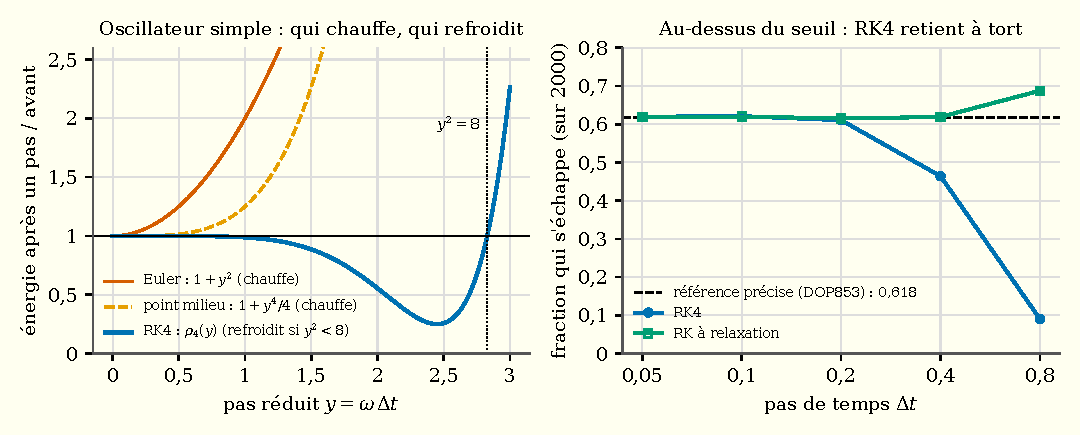
\includegraphics[width=\linewidth]{figures/c20_rk4}
\caption{À gauche~: énergie après un pas sur un ressort parfait, calculée ici et égale aux formules démontrées~;
RK4 refroidit tant que $y^2<8$. À droite~: fraction des orbites au-dessus du seuil qui s'échappent, d'après les
comptes publiés~: RK4 en retient trop aux grands pas.}
\label{fig:c20}
\end{figure}
